\documentclass[a0,portrait]{lab-poster}

\usepackage[brazil]{babel}    % Configuração de Linguagem (comentar para inglês)
% \renewcommand{\tablename}{Tabela}
% \renewcommand{\figurename}{Figura}

% \newcommand\itemadjust{\itemsep.5em \parskip0pt \parsep0pt}

\title{Mapeamento de recursos sob computação em névoa}
\author{Felipe Brizola Bergues Duro}
\major{Ciência da Computação}
% \major{Ciência da Computação/Engenharia da Computação/Engenharia Elétrica/...}
\advisor{Prof. Dr. Sérgio Johann Filho}

\themecolor{NavyBlue}
\unilogo{fig/ep-logo.pdf}
\lablogo{fig/ep-logo.pdf}

\begin{document}
\maketitle

%---------------------------------------------------------------

\begin{multicols}{2} 
%---------------------------------------------------------------
%	MOTIVAÇÃO
%---------------------------------------------------------------
% \color{NavyBlue}
\section*{Introdução}
% \color{Black}
\Large
\justifying
\begin{itemize}

\item A computação em névoa é um termo relativamente novo e teve sua primeira definição, dada pela Cisco Systems em 2012, como uma extensão do modelo de computação em nuvem que provê armazenamento, computação e serviços de rede entre dispositivos finais e os servidores na nuvem \cite{DBLP:journals/corr/RomanLM16}.
\item A computação em névoa tornou-se um paradigma próprio deixando de ser um apêndice da computação em nuvem. Deste novo paradigma surgiu o termo de \textit{fog node}, que abrange desde dispositivos finais com baixa capacidade computacional até servidores poderosos na nuvem.
\item Os problemas referentes à padronização, descoberta e sincronização são os motivadores deste trabalho, uma vez que atualmente não existem mecanismos no qual um membro da névoa, seja um dispositivo com limitações de memória e processamento ou um computador robusto, mapeiem os recursos disponíveis e divulgue os seus na rede.
\item A computação em névoa pode ser ilustrada pela imagem abaixo, na qual demonstra uma arquitetura base deste cenário.

\begin{center}
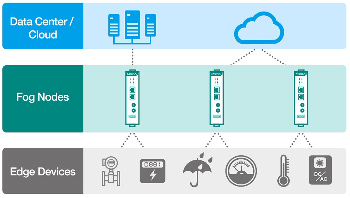
\includegraphics[width=0.7\linewidth]{fig/fig1.pdf}
\end{center}

\item Seguindo a organização arquitetural da imagem acima, a proposta deste trabalho é fazer com que um \textit{fog node} conheça, de forma autônoma e descentralizada, os recursos disponibilizados por seus vizinhos.
Assim, cada \textit{fog node} saberá quais são os \textit{edge devices} disponíveis na rede, portanto,
o nodo que possui o sensor de chuva saberia da existencia de um outro nodo na rede capaz de medir a temperatura, por exemplo.

\item A comunicação entre os \textit{fog nodes} e seus sensores, comumente chamados de \textit{edge devices}, ocorre utilizando o protocolo CoAP - Constrained Application Protocol.
\item O CoAP implementa a RFC-6690 - Constrained RESTful Environments (CoRE) Link Format - que possui como finalidade a realização de REST em nodos com recursos limitados\cite{rfc6690}.
\item CoAP também implementa a RFC-5785 que define como URI padrão o prefixo /.well-known/core. Este prefixo é utilizado para que o servidor exponha suas políticas e recursos disponíveis\cite{rfc5785}.

\end{itemize}

\section*{\huge Protocolo Proposto}

\Large
\justifying
\begin{itemize}

\item A imagem a seguir ilustra a pilha de protocolos utilizados na implementação deste projeto, bem como o detalhamento estrutural do protocolo proposto, intitulado Resource Mapping.


\begin{center}
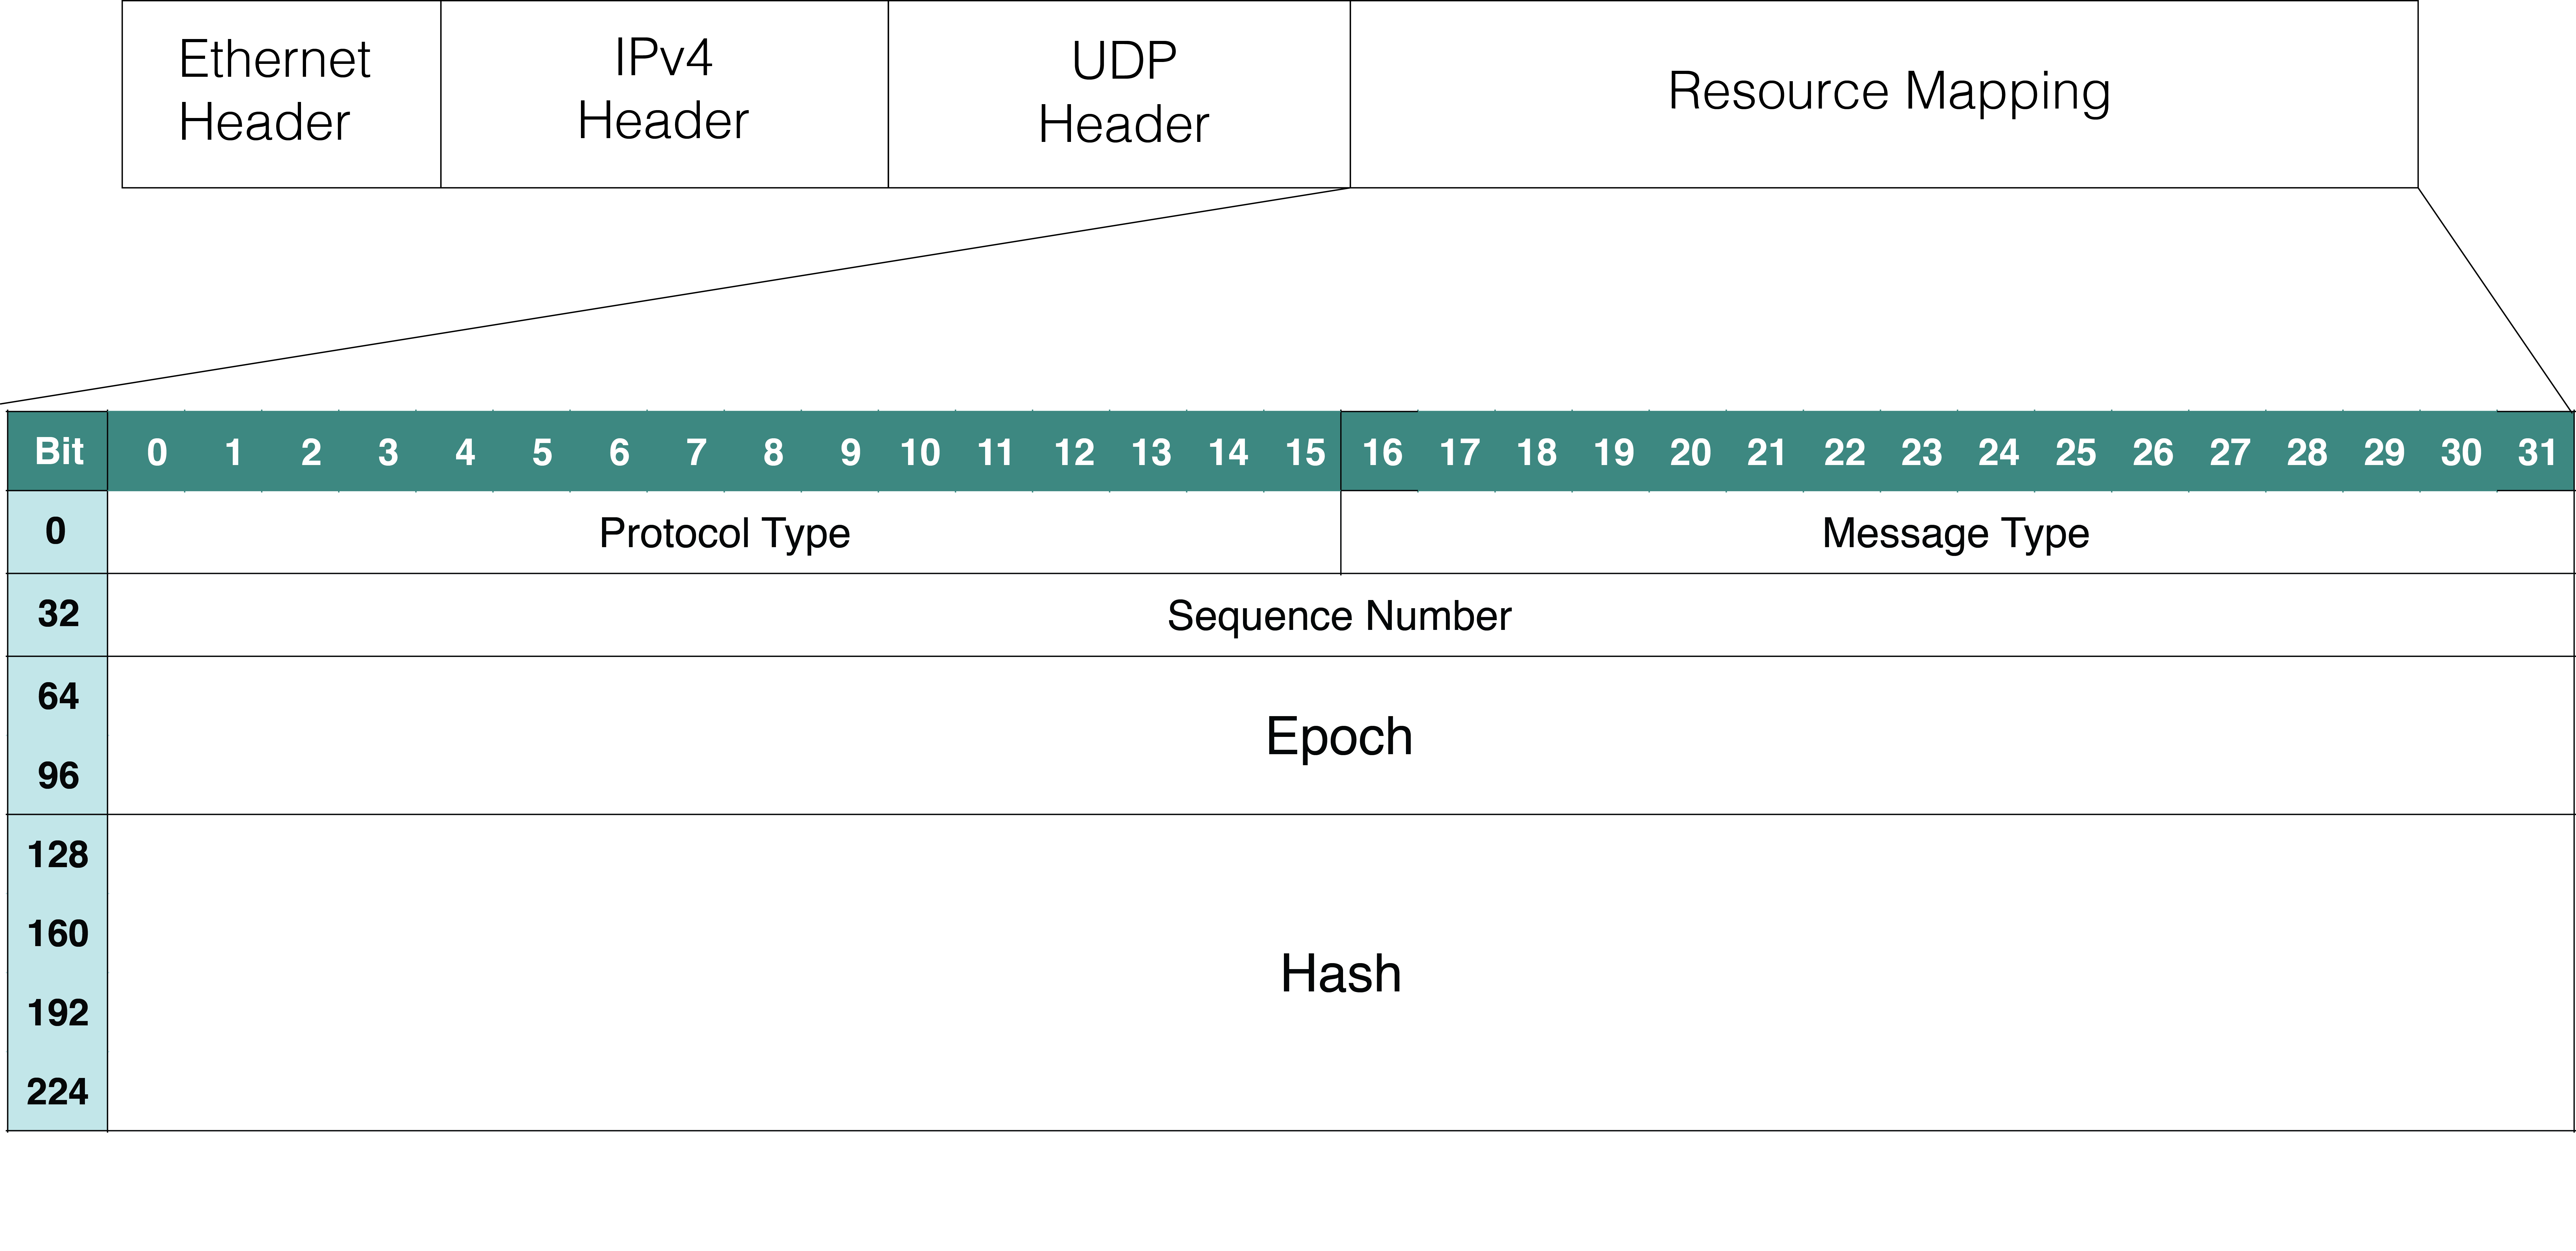
\includegraphics[width=0.7\linewidth]{fig/fig2.png}
\end{center}

\item O campo Protocol Type é reservado para indicar a forma de encapsulamento do pacote.
\item Atualmente existem dois tipos de Messages Types possíveis, keep alive e acknowledgement.
\item Sequence Number tem o intuito de identificar o pacote enviado.
\item O campo Epoch é utilizado para indicar alterações nos recursos providos pelo fog node.
Sendo assim, quando um recurso é adicionado ou removido de um fog node, o campo Epoch é acrescido em uma unidade.
\item O campo Hash utiliza a função de criptografia MD5 para validar a integridade dos demais campos contidos no pacote.
\end{itemize}



\section*{\huge Funcionamento}

\Large
\justifying
\begin{itemize}

\item Os fog nodes, a cada trinta segundos, enviam mensagens por multicast indicando que ainda estão em operação.
Essas mensagens são do tipo keep alive e carregam consigo a época em que o fog node se encontra. 
\item Ao receber as mensagens de keep alive, o fog node valida se já possui este IP mapeado em sua lista de recursos globais.
Caso não possua o IP, deverá, então, realizar uma requisição CoAP para a URI /.well-known/core a fim de obter os recursos providos pelo fog node.
Caso já possua o IP mapeado, deverá, então, verificar se a época recebida é diferente da que possui.
Havendo divergência entre as épocas, uma nova requisição CoAP para a URI /.well-known/core deverá ser realizada com o intento de atualizar a listagem de recursos providos pelo node.
\item Após receber a mensagem de keep alive e processá-la, outra mensagem, desta vez de acknowledgement, é enviada de volta ao remetente do keep alive.
Desta forma, o remetente passa a ter conhecimento que o fog node ainda está em operação.
\item Para que seja possível saber quando um membro deixou de fazer parte da névoa, o mecanismo proposto funcionada de tal forma que a cada três timeouts consecutivos de acknowledgement
o fog node é removido da lista de recursos globais.

\end{itemize}

\begin{center}
    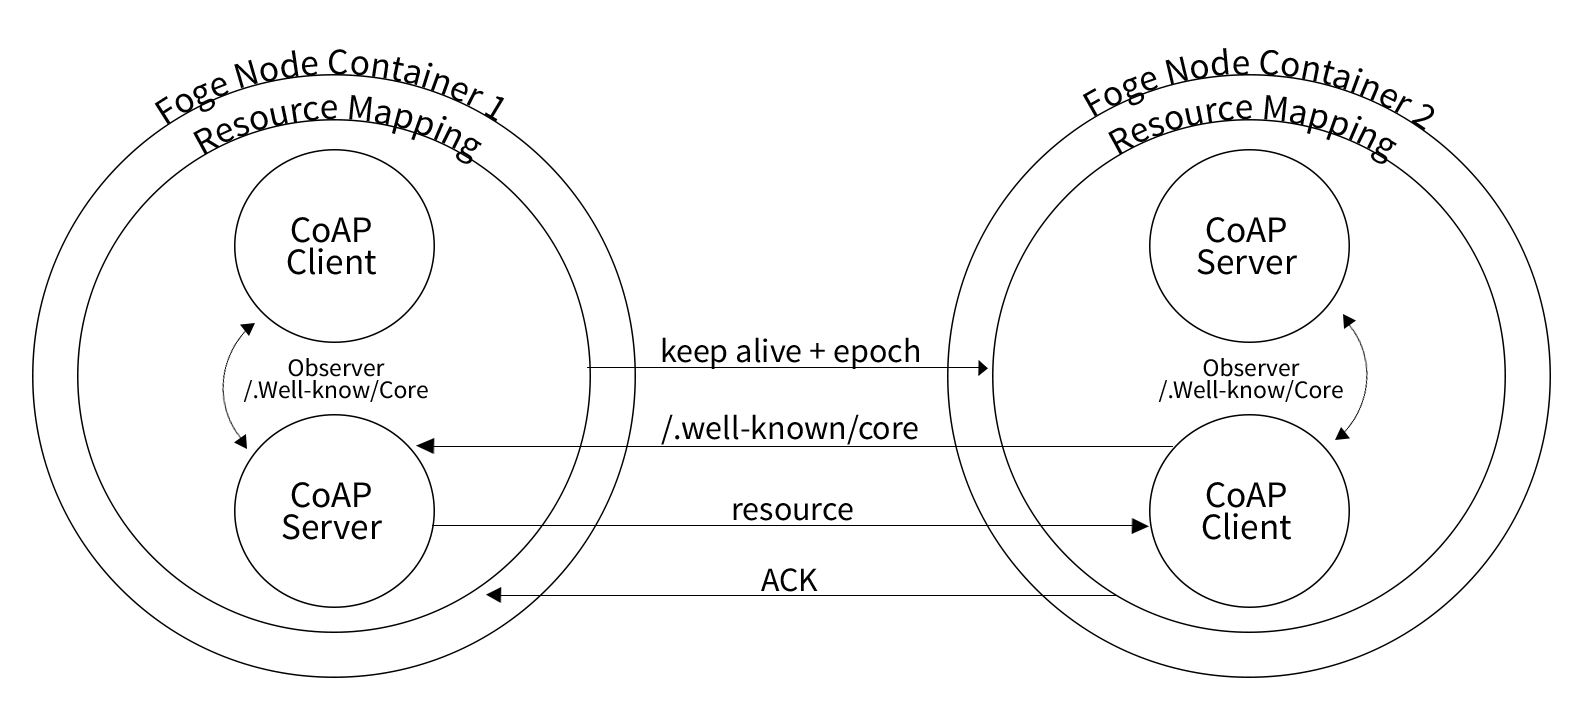
\includegraphics[width=0.7\linewidth]{fig/fig3.png}
\end{center}

\section*{\huge Experimentos}

\Large
\justifying
\begin{itemize}

\item O ambiente de testes da solução foi construído utilizando containers Docker e scripts Python.
% \item O gerenciamento dos containers na névoa é automatizado, portanto, é possível dinamicamente adicionarmos ou removermos containers da rede.
\item O gerenciamento dos containers na névoa foi automatizado, deste modo é possível adicionarmos ou removermos fog nodes dinamicamente.
\item O gerenciamento dos recursos de um determinado fog node também foi automatizado, sendo assim, é possível incluirmos ou retirarmos edge devices dinamicamente.
\item Os experimentos se mostraram satisfatórios, uma vez que foi possível criar um ambiente com quarenta fog nodes e a sincronização dos recursos transcorreu normalmente.
Esta limitação dá-se pelo fato do computador hospedeiro, que executa dos containers, não possuir recursos suficientes para a expansão da escalabilidade dos testes.



\end{itemize}
%---------------------------------------------------------------
%	REFERENCES
%---------------------------------------------------------------
% Descomentar abaixo caso queira usar referências bibliográficas no poster
\vspace{-10mm}
\large
\color{NavyBlue}
\color{Black}
\raggedright
\bibliographystyle{plain}
\bibliography{poster}

\end{multicols}

%----------------------------------------------------------------------------------------
\end{document}